\documentclass[./main.tex]{subfiles} 
\begin{document}

\section{Adaptive Signal Processing}

\subsection{The Least Mean Squares (LMS) Algorithm}

\subsubsection{Correlation Matrix}
The autocorrelation matrix is been defined as $ R \equiv E \begin{bmatrix} \mathbf{x}[n] \mathbf{x}^T[n] \end{bmatrix} $

\begin{equation}
R = E \begin{bmatrix}
x^2[n-1] & x[n-1] x[n-2] \\
x[n-1] x[n-2] & x^2[n-2]
\end{bmatrix}
\end{equation}
\label{eq:3_1_a_R}

We note that $x^2[n-1] = x^2[n-2] $ since this simply represents a shift in the time domain but will not change the expected value. 

We can square $x[n]$ to give us the expected value of the diagonals:
\begin{subequations}
\begin{align}
E[x[n-1]] &= E[ a_1 x[n - 2] + a_2 x[n-3] + \eta[n-1] ] \\
E[x^2[n-1]] &= E[ a_{1}^2 x^2[n - 2]] + E[ a_{2}^2 x^2[n-3]] + E[ 2 a_{1} a_{2} x[n-1] x[n-2]] + 
\sigma^2 \\
R_{xx}(0) = E[x^2[n-1]] &= a_1^2 R_{xx}(0) + a_2^2 R_{xx}(0) + 2 a_{1} a_{2} R_{xx}(1)
\end{align}
\end{subequations}

We get to the last line using the equality mentioned above, and we can see the make up of $R_{xx}(1)$ in equation \ref{eq:3_1_a_R}. We can conduct a similar process for $R_{xx}(1)$:

\begin{subequations}
\begin{align}
E[x[n-1]] &= E[ a_1 x[n - 2] + a_2 x[n-3] + \eta[n] ] \\
E[x[n-1]x[n-2]] &= E[ a_1 x^2[n - 2] + a_2 x[n-3]x[n-2] + \eta[n-1]x[n-2] ] \\
R_{xx}(1) = E[x[n-1]x[n-2]] &= a_1 R_{xx}(0) + a_2 R_{xx}(1) + 0
\end{align}
\end{subequations}

We then solve these two equations for $ R_{xx}(0) $ and $ R_{xx}(1) $, to determine that the autocorrelation matrix is 
$$ R = \begin{bmatrix}
\frac{25}{27} & \frac{25}{54} \\[0.3em]
 \frac{25}{54} & \frac{25}{27}
\end{bmatrix}
$$

In order for the filter to converge to the correct parameters, we must satisfy the bounds $ 0 < \mu < \frac{2}{\lambda_{max}} $. In this case, our eigenvalues are $\frac{25}{18}$ and $\frac{25}{54}$. Thus we know that $ 0 < \mu < \frac{108}{25} $ for the LMS to converge in the mean.

\subsubsection{Implemented LMS Filter}
100 iterations of the AR Process $ x[n] = 0.1 x[n-1] + 0.8 x[n-2] + \eta[n] $ have been generated, with 1000 samples per iteration. Figure \ref{fig:q3_1_b_indiv} shows one trial of this filter, whist figure \ref{fig:q3_1_b} shows the mean error taken across 100 iterations.

\begin{figure}[h]
	\centering 
 	\resizebox{\textwidth}{!}{% This file was created by matlab2tikz v0.4.7 (commit e8e34ce6bed2236de660d19205fcab087937605e) running on MATLAB 8.3.
% Copyright (c) 2008--2014, Nico Schlömer <nico.schloemer@gmail.com>
% All rights reserved.
% Minimal pgfplots version: 1.3
% 
% The latest updates can be retrieved from
%   http://www.mathworks.com/matlabcentral/fileexchange/22022-matlab2tikz
% where you can also make suggestions and rate matlab2tikz.
% 
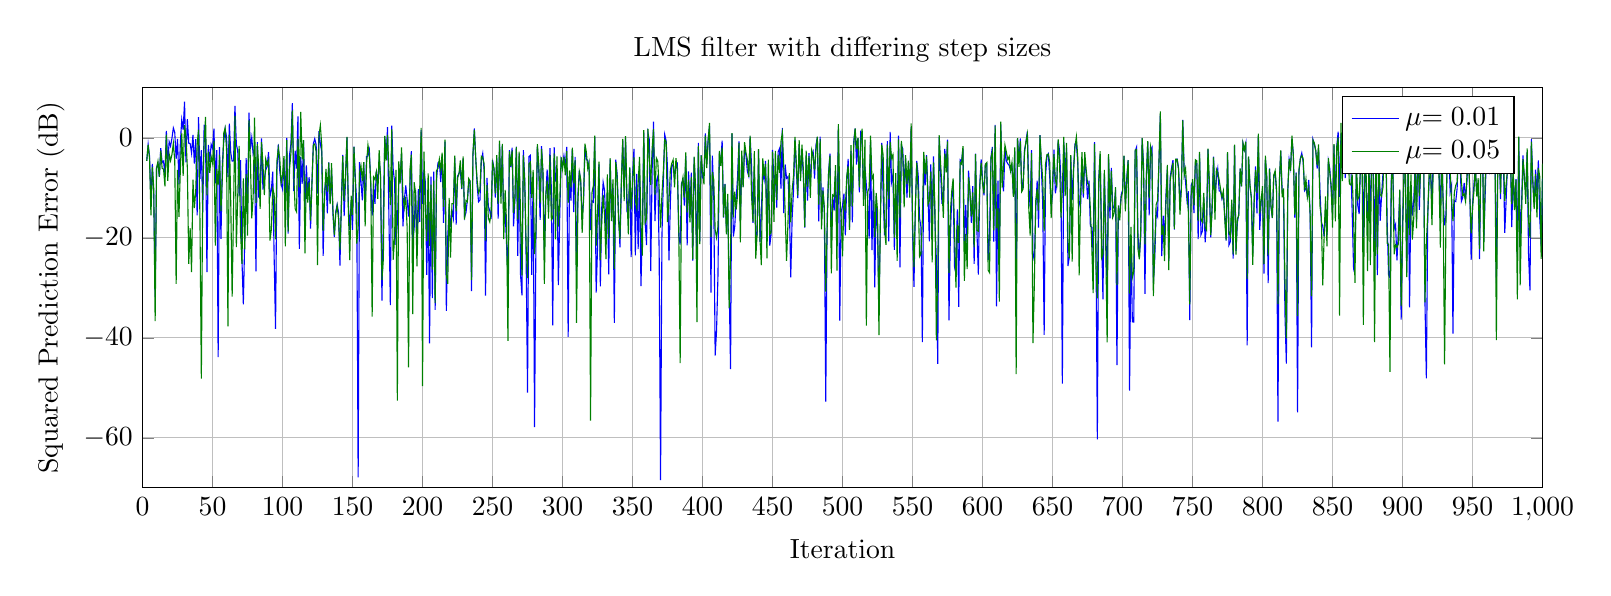
\begin{tikzpicture}

\begin{axis}[%
width=7in,
height=2in,
unbounded coords=jump,
scale only axis,
xmin=0,
xmax=1000,
xlabel={Iteration},
xmajorgrids,
ymin=-70,
ymax=10,
ylabel={Squared Prediction Error (dB)},
ymajorgrids,
title={LMS filter with differing step sizes},
legend style={draw=black,fill=white,legend cell align=left}
]
\addplot [color=blue,solid]
  table[row sep=crcr]{1	-inf\\
2	-inf\\
3	-4.59507082620591\\
4	-1.29996298596598\\
5	-3.70388331513567\\
6	-12.886796582078\\
7	-5.21161423976009\\
8	-11.4515929637692\\
9	-31.8370688452581\\
10	-5.99162122660154\\
11	-5.08424174660262\\
12	-7.79254593632003\\
13	-2.06806015100985\\
14	-4.92051303110294\\
15	-4.64612437362596\\
16	-7.36334277057199\\
17	1.40876675529917\\
18	-5.0262432391268\\
19	-0.758097027471307\\
20	-1.6496687842333\\
21	-0.077601116516787\\
22	1.97568414911764\\
23	1.10298527821058\\
24	-4.19253733201039\\
25	-0.198870346518106\\
26	-9.3095623607669\\
27	-1.01821155998611\\
28	3.6024438963203\\
29	1.6173802853813\\
30	7.22941099683327\\
31	-4.90031115684373\\
32	3.7503490465052\\
33	-1.0576737892293\\
34	-1.13233545410099\\
35	-3.03883378331891\\
36	0.573129369513038\\
37	-5.13192022683942\\
38	-0.276296218095252\\
39	-15.5128888879724\\
40	4.1398369269964\\
41	-8.17794661983596\\
42	-2.44369493494699\\
43	-14.8946763118055\\
44	2.65976655029787\\
45	-0.0394474379340101\\
46	-26.8684613523647\\
47	-1.42133766862283\\
48	-4.82857983328491\\
49	-1.30330785168854\\
50	-2.10558373460676\\
51	1.83122424331736\\
52	-9.07613523964419\\
53	-2.43586414265314\\
54	-43.8608087336864\\
55	-1.8442658460936\\
56	-20.2101840746231\\
57	-5.11221560134833\\
58	-0.739777467831388\\
59	1.75173115316697\\
60	0.231989354962519\\
61	-7.85790934623202\\
62	2.83678802826973\\
63	-2.98120455648551\\
64	-4.63760333820862\\
65	-4.60747291274579\\
66	6.38720782860191\\
67	-1.30263365227467\\
68	-2.59934307167544\\
69	-11.651066347851\\
70	-4.44070447113303\\
71	-24.3951070902113\\
72	-33.2958131455893\\
73	-20.1564571010961\\
74	-4.06092041390022\\
75	-15.2571950153253\\
76	5.03557130376121\\
77	-2.20505859308837\\
78	0.0543752516346717\\
79	-3.26661775112839\\
80	-2.30448933256956\\
81	-26.7185809941387\\
82	-0.834947144094049\\
83	-11.9348680897793\\
84	-10.1041576485053\\
85	-0.0983277583617844\\
86	-10.3460119082907\\
87	-8.24348146730097\\
88	-6.42732422694919\\
89	-5.74574071803219\\
90	-2.83501623014551\\
91	-11.7501929701949\\
92	-10.4795077260658\\
93	-6.73708069559175\\
94	-23.864291145364\\
95	-38.1993688773272\\
96	-6.09531401969005\\
97	-1.31943322728795\\
98	-6.54184797217457\\
99	-9.24243669632859\\
100	-10.2514267660012\\
101	-4.35629192220219\\
102	-13.3807838448117\\
103	0.0183787725011844\\
104	-19.152998673932\\
105	-3.43071743111616\\
106	-1.11428963801003\\
107	6.92598566526701\\
108	-10.671238192262\\
109	-2.5763252146889\\
110	-6.14809048565763\\
111	4.28900252463904\\
112	-22.1820323251344\\
113	-3.87733164372634\\
114	-9.19193006295974\\
115	-0.50820181437446\\
116	-13.6797773066692\\
117	-5.50277846404101\\
118	-11.104973275357\\
119	-7.8581784814733\\
120	-18.167470554977\\
121	-8.86388988270849\\
122	-1.17932001354982\\
123	-0.173843892636093\\
124	-1.41001109031989\\
125	-11.1351654408496\\
126	1.32609109963583\\
127	-1.16111425898\\
128	-2.76552856078371\\
129	-23.5981420714182\\
130	-10.6510614426644\\
131	-8.17233603411163\\
132	-15.07750206477\\
133	-4.91182925626672\\
134	-13.1109926636608\\
135	-6.3650256200269\\
136	-15.2076948811646\\
137	-19.8704542331295\\
138	-14.7754553992367\\
139	-13.3283581467692\\
140	-14.9293129240127\\
141	-25.5340869613823\\
142	-13.0121406171393\\
143	-3.40170879957216\\
144	-15.6306722974278\\
145	-8.3444023512049\\
146	0.0993009897631158\\
147	-13.297418621087\\
148	-18.3912674721723\\
149	-12.8095607365625\\
150	-18.4180152488787\\
151	-1.77314047203756\\
152	-8.00979329271622\\
153	-13.0798758610286\\
154	-67.8798107293025\\
155	-4.8713240947399\\
156	-8.62353014193708\\
157	-12.4956045813881\\
158	-4.8789965668519\\
159	-13.6827434845321\\
160	-3.69847656875362\\
161	-3.65416040114594\\
162	-2.47866388854382\\
163	-9.27219663908088\\
164	-15.5569454846821\\
165	-9.18269700077577\\
166	-13.2004768376506\\
167	-6.59536159387419\\
168	-9.32623776602284\\
169	-4.35391172388237\\
170	-7.45588773925131\\
171	-32.5646848152241\\
172	-15.7648371832139\\
173	0.290314107379467\\
174	-3.80533935492875\\
175	2.16206068938495\\
176	-16.2097483783635\\
177	-33.4381878005289\\
178	2.42970182112264\\
179	-6.13827213232283\\
180	-8.78183551030334\\
181	-21.4209022307097\\
182	-17.0412750064657\\
183	-8.97365984758658\\
184	-7.91276035077917\\
185	-3.21215558211807\\
186	-17.6906391102931\\
187	-12.4179301429368\\
188	-9.53250601887263\\
189	-12.2898472545387\\
190	-15.7302754663766\\
191	-9.49431646292227\\
192	-2.67296133362224\\
193	-20.7538936228713\\
194	-18.1525034084186\\
195	-10.4251631852447\\
196	-21.0081519792554\\
197	-10.254204952508\\
198	-16.7954087768511\\
199	1.57208708557949\\
200	-13.1841153849734\\
201	-6.34799004651346\\
202	-8.89470144548437\\
203	-27.4103919291639\\
204	-10.3470266018799\\
205	-41.0806085382544\\
206	-7.76301208371989\\
207	-32.0349062880966\\
208	-6.7327939113944\\
209	-34.3969084998931\\
210	-8.28871591620671\\
211	-5.01886041498538\\
212	-4.71853660706931\\
213	-8.82505129259185\\
214	-3.51010923435167\\
215	-16.9963362896896\\
216	-0.730528882716501\\
217	-34.6196189079352\\
218	-19.7688721520734\\
219	-13.8765771507028\\
220	-17.8131518378593\\
221	-14.6634275490892\\
222	-16.0848299004548\\
223	-4.02587569361607\\
224	-17.3354494602711\\
225	-7.69915922620534\\
226	-7.07420493402448\\
227	-6.43256957204218\\
228	-10.2499480993552\\
229	-4.09385110283117\\
230	-15.8624865883882\\
231	-14.954989250737\\
232	-12.5134906300228\\
233	-8.99234868899662\\
234	-8.74926368569967\\
235	-30.6635886562186\\
236	-3.49476079151981\\
237	1.87692346468992\\
238	-4.18683889744427\\
239	-9.5559126140898\\
240	-12.7853084356965\\
241	-12.4270117494065\\
242	-4.56164412282348\\
243	-3.11649965297617\\
244	-6.4640977568059\\
245	-31.5667969584002\\
246	-7.9842704350142\\
247	-13.7292998292345\\
248	-14.5424244544422\\
249	-16.2279056472344\\
250	-4.41152282722257\\
251	-6.18537695238337\\
252	-11.9244805502852\\
253	-4.10245450391466\\
254	-16.1558960757809\\
255	-1.21847923362777\\
256	-11.6163037287194\\
257	-1.40743926494729\\
258	-17.3185386950072\\
259	-14.7877704292476\\
260	-21.234889571928\\
261	-27.7414751415603\\
262	-2.44167960718865\\
263	-5.83147354970486\\
264	-1.94338610639582\\
265	-17.7195805791287\\
266	-12.1778983044332\\
267	-1.74624119572146\\
268	-23.5950554512173\\
269	-3.09265685071966\\
270	-27.4090947400917\\
271	-31.4848663903897\\
272	-2.469115747857\\
273	-8.21086296044095\\
274	-24.3761309060737\\
275	-50.9309983521741\\
276	-3.73342903937243\\
277	-3.48599763691293\\
278	-27.3803033529927\\
279	-7.9197297715811\\
280	-57.8336011979566\\
281	-20.1044662510308\\
282	-1.62924795565196\\
283	-6.52224671548055\\
284	-16.4178408997187\\
285	-1.63531266213463\\
286	-7.049154576417\\
287	-22.6913949630415\\
288	-11.7995710988729\\
289	-6.33149462795096\\
290	-13.8445162269544\\
291	-2.033115959314\\
292	-10.214550246611\\
293	-37.4794256414866\\
294	-1.85329762372136\\
295	-8.75732207127788\\
296	-6.62990334596757\\
297	-29.4376381613258\\
298	-15.4224345685412\\
299	-4.38626569475822\\
300	-5.57282360658109\\
301	-3.54999256460616\\
302	-5.60055661953875\\
303	-1.79193704050829\\
304	-39.7806079213807\\
305	-7.64824348894368\\
306	-12.5426513281241\\
307	-2.17789945825479\\
308	-14.8405457588761\\
309	-3.81946842826283\\
310	-26.663552504303\\
311	-11.1256911677689\\
312	-6.49047959791645\\
313	-9.11794370343059\\
314	-15.6892526371147\\
315	-12.7992989995148\\
316	-1.77578442645775\\
317	-4.34970961006816\\
318	-4.48446596321813\\
319	-6.12356035243434\\
320	-18.4663190660257\\
321	-12.5937084556932\\
322	-12.8499281501326\\
323	0.134504841403184\\
324	-30.9515249949078\\
325	-22.0388073875331\\
326	-5.28875253141051\\
327	-29.723246827461\\
328	-13.9147915126818\\
329	-8.88979378957893\\
330	-10.5320046110287\\
331	-18.5165653404073\\
332	-11.0609292076673\\
333	-27.3054484804337\\
334	-4.28227567648723\\
335	-14.9241250826485\\
336	-10.0043263230464\\
337	-37.0130881420234\\
338	-4.37246630658153\\
339	-7.26399436249821\\
340	-14.8434148010706\\
341	-21.8793792859966\\
342	-9.45580093095956\\
343	-0.559489052786781\\
344	-10.626668027507\\
345	0.0129315707530535\\
346	-14.6851468194501\\
347	-15.3193374109357\\
348	-6.12558360255809\\
349	-23.8503853354557\\
350	-7.6322770221229\\
351	-2.21046023269715\\
352	-23.5146177835239\\
353	-7.22302901743624\\
354	-22.2691387721479\\
355	-6.26649583247766\\
356	-29.6443851567446\\
357	-18.2473211824487\\
358	1.04982984971172\\
359	-16.6178353037298\\
360	-21.4331081748009\\
361	0.971111150022873\\
362	-0.386985153461473\\
363	-26.6260658910693\\
364	-6.21568263451509\\
365	3.24528470398526\\
366	-16.654678204431\\
367	-8.74410983119098\\
368	-7.73779060519475\\
369	-22.5970694892614\\
370	-68.4469019816751\\
371	-19.5353467588415\\
372	-8.59866069349975\\
373	0.658040388164451\\
374	-0.609359314445117\\
375	-6.34160738146867\\
376	-24.524191047539\\
377	-13.0186888297633\\
378	-5.29764461668775\\
379	-5.61178920306852\\
380	-8.02663249324909\\
381	-4.80507716175149\\
382	-5.0367922652333\\
383	-19.600287390056\\
384	-21.3555994885052\\
385	-9.11700423261428\\
386	-8.38759234391449\\
387	-13.5354160994604\\
388	-3.63369643485395\\
389	-21.5215489864056\\
390	-6.69524651519009\\
391	-14.0352044412132\\
392	-6.97299698142079\\
393	-24.5437723342562\\
394	-3.89794360118936\\
395	-11.4007279363398\\
396	-24.8635622808819\\
397	-0.989728166179697\\
398	-20.7151684821471\\
399	-3.44957700946648\\
400	-7.89217444923396\\
401	-7.4512907946588\\
402	0.897049616552637\\
403	-5.21647046361236\\
404	-0.260277362193214\\
405	2.35688640880273\\
406	-30.9401730031022\\
407	-3.55742416368125\\
408	-11.296960226021\\
409	-43.5575009659946\\
410	-38.5716970565132\\
411	-27.6790599041766\\
412	-3.65044722916638\\
413	-4.74205554608764\\
414	-0.546083345850634\\
415	-15.9279673627633\\
416	-9.215540787427\\
417	-17.9939008396808\\
418	-12.9298854771972\\
419	-29.4591632173433\\
420	-46.2324028684693\\
421	0.872144235007382\\
422	-19.7383201399374\\
423	-17.7338618408133\\
424	-12.3400541916129\\
425	-7.91933368859598\\
426	-0.724951334866135\\
427	-16.9438322294593\\
428	-3.87322146809172\\
429	-9.77766156164657\\
430	-2.2799497575516\\
431	-3.46232804437846\\
432	-6.66975950021396\\
433	-7.64343244956849\\
434	0.265543639754774\\
435	-5.61272342064353\\
436	-17.0005461011555\\
437	-6.43514883117215\\
438	-19.3293337078133\\
439	-19.4102556923633\\
440	-2.51619356556718\\
441	-20.8157786757831\\
442	-15.059990349752\\
443	-6.50971397149091\\
444	-8.36142565433981\\
445	-4.60492032628457\\
446	-16.8329011943879\\
447	-7.31184564338407\\
448	-21.5554017203759\\
449	-19.2287822796231\\
450	-2.41758081503257\\
451	-8.68711230220087\\
452	-7.40243215603317\\
453	-13.9690477824568\\
454	-2.81684443908056\\
455	-2.12802720993685\\
456	-10.1360977786818\\
457	1.95712346627217\\
458	-15.0495361171828\\
459	-5.33223691626302\\
460	-8.0822792755122\\
461	-7.75011648932619\\
462	-13.5099209237612\\
463	-27.9051087369194\\
464	-15.9524237906848\\
465	-10.4588298894738\\
466	-0.374689457951622\\
467	-6.34337401071064\\
468	-12.0623033859673\\
469	-1.28982523731276\\
470	-7.15720053986975\\
471	-3.20341640882774\\
472	-7.33437632689617\\
473	-17.9611041005778\\
474	-3.46930370543498\\
475	-12.5538046795972\\
476	-3.04101371975908\\
477	-9.20069732172808\\
478	-3.42541422572739\\
479	-2.72345271534146\\
480	-8.1282286315345\\
481	-1.47244212886749\\
482	0.165360741722727\\
483	-16.6788900603673\\
484	0.231182230266583\\
485	-16.3361804489302\\
486	-9.91726254832736\\
487	-15.0525583598902\\
488	-52.736230493891\\
489	-15.9025058786515\\
490	-7.09745032673951\\
491	-3.15318036805746\\
492	-20.4031897042768\\
493	-12.1211281856933\\
494	-14.5585372286106\\
495	-6.56361969993684\\
496	-21.6914194284372\\
497	2.30577660084875\\
498	-36.5417851588361\\
499	-14.8862425900649\\
500	-13.553063569923\\
501	-11.1677813226703\\
502	-19.4993084004511\\
503	-8.82882928953749\\
504	-4.19438031309641\\
505	-17.8844070629149\\
506	-2.59151300868696\\
507	-16.9236679856363\\
508	-0.675193300907349\\
509	1.88587207518606\\
510	-5.36833986435831\\
511	-0.0793074678597081\\
512	-10.9236823934515\\
513	1.45550837958505\\
514	-0.534628893516546\\
515	-12.3578339926104\\
516	-5.76091845114609\\
517	-9.52070462835327\\
518	-12.5817098473138\\
519	-20.1353251137388\\
520	-0.802415503968789\\
521	-22.4292581952875\\
522	-9.70623806421799\\
523	-29.8830562945552\\
524	-12.3852365333921\\
525	-18.6945553783361\\
526	-33.6681236101592\\
527	-16.9900999118575\\
528	-0.98826968257937\\
529	-11.3127525522308\\
530	-19.5113562055399\\
531	-17.3357776437433\\
532	-0.662976499796476\\
533	-20.6960983566777\\
534	1.18241613941875\\
535	-8.8483314372485\\
536	-7.32567828000341\\
537	-22.3929193286133\\
538	-10.3549318399844\\
539	-16.3921167422206\\
540	0.427262662927257\\
541	-25.915192160491\\
542	-1.49110748064582\\
543	-2.15340805225087\\
544	-10.1474938055881\\
545	-4.1843469410761\\
546	-11.9379434547792\\
547	-6.26552474038482\\
548	-9.59247387633391\\
549	2.20195331066449\\
550	-18.5020963264594\\
551	-29.7902137673919\\
552	-13.9246526150587\\
553	-4.62523513605747\\
554	-7.37978008342056\\
555	-16.0022217032059\\
556	-17.8437548839065\\
557	-40.8499429725252\\
558	-4.16729394634423\\
559	-9.49467327740707\\
560	-3.46590601116439\\
561	-10.8928012272757\\
562	-20.6787521170659\\
563	-5.29407695733245\\
564	-16.1331892141887\\
565	-3.69063125136237\\
566	-16.7291949328809\\
567	-24.2655731632478\\
568	-45.1990754893354\\
569	0.21564712498018\\
570	-6.64938166389886\\
571	-13.0748326518308\\
572	-13.0333927112635\\
573	-2.19516267469937\\
574	-5.70059092339742\\
575	-0.373631043128781\\
576	-36.5146418793694\\
577	-19.6479513644404\\
578	-11.7898198657758\\
579	-10.1362244368425\\
580	-25.7758032144352\\
581	-24.5261808678046\\
582	-14.3108058437029\\
583	-33.7827437338014\\
584	-4.38370901604128\\
585	-4.696611564589\\
586	-2.14597081163304\\
587	-21.2824734665391\\
588	-13.4139804491998\\
589	-21.5132214997234\\
590	-6.54955776991532\\
591	-11.0304129524087\\
592	-17.0039565329184\\
593	-9.67566721990508\\
594	-25.2213423353637\\
595	-3.15577201111082\\
596	-18.8012498438855\\
597	-27.3356929352686\\
598	-9.36178372481423\\
599	-4.31882950045207\\
600	-8.18885990064409\\
601	-11.500618311346\\
602	-5.25989999620003\\
603	-5.1209923676764\\
604	-24.4689185127553\\
605	-19.3451633902022\\
606	-3.90232909110674\\
607	-1.82495683575589\\
608	-20.7445917670522\\
609	2.60214879808498\\
610	-33.7026016949724\\
611	-8.55984408215417\\
612	-24.3773878599658\\
613	2.67481913141908\\
614	-8.04829502870602\\
615	-10.7131109205548\\
616	-2.21994930949284\\
617	-4.63342635330954\\
618	-5.16146592636558\\
619	-5.5056959861348\\
620	-6.51934413895587\\
621	-5.76501882836911\\
622	-11.2498070433476\\
623	-2.72743083063992\\
624	-27.8665008291221\\
625	-0.0460309354229173\\
626	-4.77707988123796\\
627	-0.106019430403927\\
628	-10.6931977103372\\
629	-8.77322200558055\\
630	-2.39052052340704\\
631	-0.860753105377968\\
632	1.28309260465083\\
633	-9.75262256063659\\
634	-13.8990147954204\\
635	-2.44759493218307\\
636	-22.8747611432918\\
637	-24.6198767777989\\
638	-14.180229789774\\
639	-8.55821588842579\\
640	-17.9598514102633\\
641	0.546662586103071\\
642	-5.71005430277453\\
643	-13.3639977267362\\
644	-39.377367331802\\
645	-7.58698602430216\\
646	-3.67740752506266\\
647	-3.20493029884051\\
648	-7.93883080994749\\
649	-13.707906963565\\
650	-11.3612045182486\\
651	-2.37501062159097\\
652	-11.0871713996218\\
653	-9.2854770358682\\
654	-0.531674703725932\\
655	-2.60907737100782\\
656	-8.82012957296071\\
657	-49.1391243602649\\
658	-0.812776840688331\\
659	-7.4105446744849\\
660	-1.96458770625016\\
661	-25.6222629761917\\
662	-23.7875778706937\\
663	-3.68352296914962\\
664	-12.4644485081821\\
665	-6.21894508125936\\
666	-1.20082007788518\\
667	-0.962267292520901\\
668	-5.10437719077415\\
669	-12.629323687721\\
670	-14.1851475916404\\
671	-4.14802226665101\\
672	-11.9715957016192\\
673	-4.10351074135163\\
674	-7.21771255642613\\
675	-12.268647168562\\
676	-8.56932778637795\\
677	-17.6370971721141\\
678	-17.9048046751993\\
679	-23.3217875906554\\
680	-0.847359566010394\\
681	-21.2719645195621\\
682	-60.2872226268619\\
683	-8.29742345422051\\
684	-3.407647963499\\
685	-18.898589906062\\
686	-32.2887938828777\\
687	-7.17573433357689\\
688	-17.4325618597089\\
689	-30.9071306661163\\
690	-3.80491729268702\\
691	-16.091394979948\\
692	-6.02606294333236\\
693	-14.0831444352752\\
694	-13.7656523641815\\
695	-10.4196704586103\\
696	-45.4496947136098\\
697	-14.647601677602\\
698	-14.8490545704509\\
699	-11.406881629348\\
700	-10.5052066529088\\
701	-3.63981753118687\\
702	-13.2705915324122\\
703	-8.0560655095546\\
704	-4.43214208764918\\
705	-50.5544555274426\\
706	-20.3690360226966\\
707	-36.7913118218173\\
708	-36.8442313361972\\
709	-2.7019488115564\\
710	-1.88270607471151\\
711	-19.3084906286311\\
712	-23.9180826458147\\
713	-19.5839281206052\\
714	-0.0638306444151733\\
715	-5.47793593706412\\
716	-31.2041491563823\\
717	-7.3880614766559\\
718	-0.841281836470773\\
719	-15.4781246708101\\
720	-2.58709597861359\\
721	-1.90715842477167\\
722	-29.0206277804334\\
723	-24.1407668148824\\
724	-14.7595032835462\\
725	-15.672335014078\\
726	-4.97009838078053\\
727	4.72584191105194\\
728	-23.659522930827\\
729	-15.5538226471643\\
730	-20.183961975916\\
731	-11.4721808264571\\
732	-6.24582401237984\\
733	-24.6282704116852\\
734	-7.9467709981083\\
735	-6.02937690697716\\
736	-4.45809498620422\\
737	-18.3343304071313\\
738	-4.32497257075085\\
739	-4.23348452155043\\
740	-6.05876509473208\\
741	-12.9873169964266\\
742	-10.0912718854086\\
743	3.60017366562059\\
744	-6.59614202218373\\
745	-8.82494167706176\\
746	-12.3985295316366\\
747	-10.681205032099\\
748	-36.4557746969611\\
749	-9.50006243693912\\
750	-8.84017048917901\\
751	-15.0676690872674\\
752	-5.18994345226683\\
753	-5.15311602335731\\
754	-20.2494998031959\\
755	-3.2342799362131\\
756	-19.3778778950083\\
757	-18.6495168473909\\
758	-12.2248409493913\\
759	-20.877713886758\\
760	-16.9172807507283\\
761	-2.29091748453994\\
762	-11.1202257346544\\
763	-19.9187631772133\\
764	-13.0324489583401\\
765	-3.73697272830864\\
766	-11.9076294316095\\
767	-8.25420428505338\\
768	-6.22370294596167\\
769	-10.5934192790391\\
770	-10.7083915268122\\
771	-12.2099152678932\\
772	-11.1268965976492\\
773	-15.3729605151294\\
774	-20.5262560191455\\
775	-3.11443250109137\\
776	-21.4239723491401\\
777	-20.752864725572\\
778	-13.1257918473029\\
779	-24.1402280792833\\
780	-1.506044175179\\
781	-22.5845911250578\\
782	-17.0157681432203\\
783	-15.195934866191\\
784	-6.15483500098634\\
785	-9.69742249219843\\
786	-1.0860289250597\\
787	-2.41322128571153\\
788	-1.10784257863776\\
789	-41.5186559346989\\
790	-3.81723413200787\\
791	-9.72281125182486\\
792	-11.8516315501663\\
793	-23.0787079651568\\
794	-12.1903408662244\\
795	-5.70091236202487\\
796	-15.0938395101\\
797	0.578222088518463\\
798	-18.4146808798088\\
799	-12.6976597489231\\
800	-11.0730197569496\\
801	-27.1259581061581\\
802	-4.16398921280157\\
803	-7.92224760197592\\
804	-29.0648320202586\\
805	-6.09728173766079\\
806	-13.7519595204771\\
807	-16.0227524254088\\
808	-7.61226477629435\\
809	-6.97369875239858\\
810	-10.909398716033\\
811	-56.7486739629067\\
812	-9.07117992578118\\
813	-2.62376276491868\\
814	-10.6657364954755\\
815	-11.9753894576029\\
816	-35.2428967000281\\
817	-45.1378482954776\\
818	-10.8830975677435\\
819	-4.31360434375807\\
820	-5.99950171596422\\
821	-0.146548592325492\\
822	-3.22603550239695\\
823	-15.9492152927238\\
824	-6.89404754108646\\
825	-54.9016715595809\\
826	-6.75909899208151\\
827	-4.10768954887973\\
828	-3.0477948908875\\
829	-4.77400475458634\\
830	-10.5164585977358\\
831	-9.98373210971098\\
832	-11.6247732227972\\
833	-8.39321728085528\\
834	-15.6362593810959\\
835	-41.8987183088764\\
836	-0.29743050989059\\
837	-1.25362111044453\\
838	-2.59583525212469\\
839	-6.1310247203147\\
840	-2.07564473836726\\
841	-10.5274437974892\\
842	-16.9461023355976\\
843	-17.6222785063779\\
844	-19.7397553882098\\
845	-14.1784921953298\\
846	-19.4454351807601\\
847	-4.63511650852455\\
848	-6.10736167245652\\
849	-10.2517724265599\\
850	-15.2978404155054\\
851	-1.49237802784727\\
852	-12.6908673274078\\
853	-1.73280273592451\\
854	1.24964853852174\\
855	-11.7841980654995\\
856	0.88554057250382\\
857	-7.56419842353094\\
858	3.84972522369639\\
859	-8.04168376860595\\
860	-3.89386920586679\\
861	-0.376439150737182\\
862	-6.92170658383385\\
863	-4.67529079198349\\
864	-14.7457267174585\\
865	-25.9971402672214\\
866	-24.744002519574\\
867	-6.15384308083854\\
868	-13.4669118047987\\
869	-15.2436952922012\\
870	-4.65681004531446\\
871	-0.844775907259722\\
872	-19.8766345121016\\
873	-5.57507640654159\\
874	-10.0770332376564\\
875	-16.8228116534975\\
876	-5.8128103038565\\
877	-16.42366518625\\
878	-0.328804284626989\\
879	-5.92654032262646\\
880	-22.5152758218973\\
881	-1.93479321101742\\
882	-27.4715076752673\\
883	-3.4268189524622\\
884	-16.5935005955718\\
885	-11.575734581961\\
886	-7.12955351458329\\
887	-2.40400750371505\\
888	0.455237192724473\\
889	-16.7474871094011\\
890	-27.399067156379\\
891	-27.9777843999778\\
892	-7.62086623272617\\
893	-5.61019089383028\\
894	-18.1782755087547\\
895	-17.3209343147756\\
896	-24.5018521070744\\
897	-18.485411307978\\
898	-10.7255978536476\\
899	-36.3474017774684\\
900	-17.2237008117576\\
901	-7.13204996950117\\
902	-7.12881250870926\\
903	-26.9466912512561\\
904	-4.74273227952773\\
905	-33.8917549988368\\
906	-9.57843848116488\\
907	-15.5299666485008\\
908	-12.5833435962541\\
909	-5.19864684832622\\
910	-16.7954317271688\\
911	1.38891463043547\\
912	-14.3941225507914\\
913	-4.20242269789914\\
914	-1.87130823648423\\
915	-1.30233266861748\\
916	-32.7110024266558\\
917	-48.1139399074848\\
918	-15.4262242800438\\
919	-8.21256431894783\\
920	-7.00239926594918\\
921	-12.0707132785045\\
922	-4.21465001959859\\
923	0.199563852351083\\
924	-5.54398814265797\\
925	-0.074545754314266\\
926	-5.86280367670915\\
927	-16.4944504538956\\
928	-2.06868164353078\\
929	-12.7816041228051\\
930	-17.4821381176137\\
931	-15.4685993169987\\
932	-3.28195073188086\\
933	-0.87030034484847\\
934	-10.8138984471462\\
935	-9.45310174584752\\
936	-39.1381733359646\\
937	-12.5863569709094\\
938	-12.7437881641295\\
939	-10.0220544285688\\
940	-0.991895352323719\\
941	-3.73022027509492\\
942	-12.7096285895359\\
943	-11.8810503254168\\
944	-8.99087315495845\\
945	-12.3068004378187\\
946	-8.69271647385258\\
947	-1.79689518009189\\
948	-10.3715276426507\\
949	-24.385657164602\\
950	-13.48936715753\\
951	-9.3081673499024\\
952	-5.67023881708189\\
953	-11.6131594391442\\
954	-9.21034538076326\\
955	-24.2592186563736\\
956	-1.5465117318502\\
957	2.70059098279195\\
958	-20.7342034483698\\
959	-11.4325332370716\\
960	-2.82912554566308\\
961	-6.00707309555652\\
962	-6.97967062516651\\
963	-6.07534955409442\\
964	-3.31416229516291\\
965	-4.10300278709956\\
966	-1.686126169691\\
967	-29.1085913872537\\
968	-4.77005215793253\\
969	-1.51697610744189\\
970	-12.2371411408001\\
971	2.77016924141861\\
972	-3.64569419734517\\
973	-19.0213271755779\\
974	-12.3396395265381\\
975	-4.85512168993333\\
976	-2.90044109484209\\
977	-2.3914242639461\\
978	-17.8440074963458\\
979	-6.91111152274734\\
980	-13.8323963121408\\
981	-8.26126886982167\\
982	-23.8106021583693\\
983	0.116480862914406\\
984	-21.4993684842843\\
985	-13.3502720453196\\
986	-3.51602226621598\\
987	-8.79460827767137\\
988	-10.7562778673912\\
989	-2.82471389601408\\
990	-23.3938012529745\\
991	-30.4773383605695\\
992	-0.260981873413256\\
993	-8.15643701935614\\
994	-13.3094085602614\\
995	-6.34532437022929\\
996	-11.0000153645085\\
997	-4.52800973464938\\
998	-16.1211463794457\\
999	-21.6858415271401\\
1000	-8.11192624795476\\
};
\addlegendentry{$\mu\text{ = 0.01}$};

\addplot [color=black!50!green,solid]
  table[row sep=crcr]{1	-inf\\
2	-inf\\
3	-4.59507082620591\\
4	-1.35734217500984\\
5	-4.1785579429237\\
6	-15.4882582479675\\
7	-5.79746890509494\\
8	-10.0945014897427\\
9	-36.6582603683893\\
10	-6.16217829452762\\
11	-4.70037976651129\\
12	-7.73513070450502\\
13	-2.55727339940239\\
14	-6.11597643687771\\
15	-6.23115034702405\\
16	-9.70296947522464\\
17	0.659237839397513\\
18	-8.61927791136672\\
19	-3.18944649045797\\
20	-4.56495132621418\\
21	-3.34296258807854\\
22	-1.09340784275436\\
23	-4.53163310655314\\
24	-29.2250198220314\\
25	-6.41061825184285\\
26	-15.8181711735545\\
27	-6.37135942672975\\
28	0.891518850590592\\
29	-7.61706453945129\\
30	2.53091770945137\\
31	0.260256281112155\\
32	-6.03838384343733\\
33	-25.2012750984346\\
34	-18.0708993487616\\
35	-26.8585833711622\\
36	-8.37681248491968\\
37	-14.0624423604493\\
38	-10.6010611884524\\
39	-1.39443096023526\\
40	1.66360945365588\\
41	-16.0914222856644\\
42	-48.1468515121566\\
43	-9.69907433239344\\
44	-1.02392425044202\\
45	4.20506522212205\\
46	-11.5204554009926\\
47	-2.75883730008218\\
48	-7.01018421917729\\
49	-3.70998156025141\\
50	-5.02787167362782\\
51	-0.580447765458768\\
52	-21.5678455739837\\
53	-6.19530644092885\\
54	-9.42373099472917\\
55	-3.38029242182558\\
56	-14.6676000519054\\
57	-7.94374498810222\\
58	0.927606839227459\\
59	2.00436401045726\\
60	-2.39857523604675\\
61	-37.7212851814447\\
62	0.643634365963009\\
63	-12.9809281655155\\
64	-31.7625667434322\\
65	-14.1270163426806\\
66	4.375364762835\\
67	-21.8677084637652\\
68	-11.5328836288984\\
69	-1.59300871614955\\
70	-18.9728738022625\\
71	-25.1966031751035\\
72	-8.11338275348861\\
73	-22.2773644112907\\
74	-7.2437081668061\\
75	-19.5738342188291\\
76	3.51405486664345\\
77	-4.30272144817998\\
78	-16.1006545728973\\
79	-11.801171402192\\
80	4.04697120109944\\
81	-12.9868426192787\\
82	-1.27628494128915\\
83	-5.99619625724916\\
84	-14.2202238831153\\
85	-0.876330815541358\\
86	-5.20369894485499\\
87	-11.4362283906375\\
88	-4.22279536389333\\
89	-5.48268014999452\\
90	-4.48263784777527\\
91	-20.5444927709623\\
92	-18.370803520996\\
93	-10.2118551915964\\
94	-11.226330548116\\
95	-20.3210629726897\\
96	-4.6239645960847\\
97	-2.05222857167635\\
98	-4.04231898735486\\
99	-9.02733958318167\\
100	-7.49110607279952\\
101	-3.66837674233741\\
102	-21.6954649310081\\
103	-0.451686620560484\\
104	-18.7594757895321\\
105	-6.25982037298366\\
106	-2.94121813267502\\
107	5.49008556039433\\
108	-7.4599478819391\\
109	-14.1646066152317\\
110	-14.7832136775484\\
111	-0.1851548977429\\
112	-9.9128354812148\\
113	5.17673917070244\\
114	-4.27456974971579\\
115	-0.436700553771977\\
116	-23.0915234825765\\
117	-7.80639799985374\\
118	-12.9291855655158\\
119	-8.82970762376246\\
120	-16.5649542474691\\
121	-9.22180350172097\\
122	-1.43101708489579\\
123	-1.22401995017946\\
124	-2.75019022738489\\
125	-25.4720631988695\\
126	0.462298038020348\\
127	2.50566040702403\\
128	-1.48040732902124\\
129	-18.6121771809577\\
130	-12.1263711738437\\
131	-6.18451443596769\\
132	-10.7704170480284\\
133	-4.96888751402041\\
134	-13.2589996478221\\
135	-5.04098339137527\\
136	-14.3525462804553\\
137	-19.4372458370727\\
138	-15.2081577809048\\
139	-13.5716920534945\\
140	-16.2475392287406\\
141	-22.3668809736861\\
142	-14.130709213483\\
143	-3.64457819301914\\
144	-12.6386519788793\\
145	-7.28529872203529\\
146	0.216869471891315\\
147	-14.3169626255634\\
148	-24.443648871851\\
149	-11.5520713450712\\
150	-15.40895332197\\
151	-1.8074177057505\\
152	-9.02006058948909\\
153	-21.1665735240365\\
154	-18.0787299891932\\
155	-6.96356781349161\\
156	-5.53774505549322\\
157	-8.65023253006201\\
158	-4.84104588274018\\
159	-17.7056854231661\\
160	-5.16919316788342\\
161	-1.4292269180782\\
162	-3.44296609676161\\
163	-8.73354622978115\\
164	-35.7309196056227\\
165	-7.81292096461944\\
166	-8.29491584711272\\
167	-6.82100509391058\\
168	-12.2214555512933\\
169	-2.43492398286348\\
170	-8.1640669169614\\
171	-28.3853687222126\\
172	-24.2693471121157\\
173	0.407234096591806\\
174	-4.56286808481747\\
175	0.578584533306172\\
176	-6.6147869196041\\
177	-13.459138285397\\
178	1.71150862978638\\
179	-24.3970789357776\\
180	-20.3289896753413\\
181	-6.39246869590977\\
182	-52.5552840214267\\
183	-4.68857930971658\\
184	-9.14254868814882\\
185	-1.91537912773946\\
186	-11.6362735777628\\
187	-13.9170762886807\\
188	-11.7453283673937\\
189	-18.0072027634916\\
190	-45.8804369931653\\
191	-6.30152082822527\\
192	-3.36319946191904\\
193	-35.2324670445659\\
194	-8.87386512724402\\
195	-10.9561408540414\\
196	-25.7087949457986\\
197	-13.4581738530941\\
198	-10.0558828624315\\
199	2.01125665685053\\
200	-49.6707893943679\\
201	-2.7741420147616\\
202	-13.7437914539626\\
203	-20.6604464218739\\
204	-7.08009984872178\\
205	-21.6028212967371\\
206	-9.3556649052998\\
207	-26.3462800025506\\
208	-8.56424165509487\\
209	-33.0504876751984\\
210	-6.56265996206758\\
211	-6.10475239194345\\
212	-4.26398072408504\\
213	-6.46553378796857\\
214	-2.95659387617396\\
215	-13.8071509300794\\
216	-0.367729700716515\\
217	-27.3896573905136\\
218	-29.2018531884668\\
219	-12.0236795193014\\
220	-23.9429136842993\\
221	-13.1539557781393\\
222	-13.1702422069474\\
223	-3.57299710611058\\
224	-14.7073949090995\\
225	-8.00863972735803\\
226	-7.23648579246877\\
227	-4.51455272901917\\
228	-10.0928839534816\\
229	-3.7245235753831\\
230	-16.3686742290434\\
231	-12.5314627077216\\
232	-12.7815480814578\\
233	-8.13575485622651\\
234	-8.67234495788636\\
235	-28.4616695184657\\
236	-3.04403400702623\\
237	1.60235375094648\\
238	-4.25736179522029\\
239	-8.53775228237179\\
240	-11.0079377878524\\
241	-10.2752947243485\\
242	-3.67730688412839\\
243	-3.89998138361175\\
244	-5.22870235737981\\
245	-20.5716559816827\\
246	-9.46139888677341\\
247	-16.0043258821735\\
248	-16.8255182111402\\
249	-14.9342483737221\\
250	-4.91768719614599\\
251	-6.12714454855965\\
252	-11.1612299361225\\
253	-3.44055873927853\\
254	-13.1773145643429\\
255	-0.57348110552321\\
256	-13.1334779188662\\
257	-1.21433602814426\\
258	-20.2516669316134\\
259	-10.4283561993743\\
260	-16.9651180607501\\
261	-40.6230511122499\\
262	-2.6904619745787\\
263	-5.63225797270658\\
264	-2.4928149082017\\
265	-14.9751787794063\\
266	-11.9690614180035\\
267	-1.85772592435593\\
268	-16.314353969406\\
269	-2.74254984439743\\
270	-15.5100822626946\\
271	-27.5205147676591\\
272	-3.5266087342012\\
273	-9.10255032440229\\
274	-21.5494620537668\\
275	-28.068837721726\\
276	-5.19117090154681\\
277	-4.85407982230267\\
278	-12.0183079805977\\
279	-6.3898833204246\\
280	-23.2674860380746\\
281	-18.4068731615398\\
282	-1.23350950068582\\
283	-5.23371476526596\\
284	-13.0826612299333\\
285	-2.25962506695624\\
286	-6.87442043086551\\
287	-29.2187555728943\\
288	-11.6176533408912\\
289	-8.5194928528505\\
290	-16.130723381405\\
291	-3.48143481578629\\
292	-16.3981987955334\\
293	-16.0478647116657\\
294	-3.12454466105426\\
295	-20.3125801051487\\
296	-3.68918189364924\\
297	-17.7253029894975\\
298	-12.6331817945499\\
299	-3.86070403935482\\
300	-6.19262459173337\\
301	-3.86223306875394\\
302	-7.50229782707988\\
303	-2.65290699879516\\
304	-13.066570266412\\
305	-6.53223912911043\\
306	-9.95273604521355\\
307	-1.95549622477469\\
308	-9.10866987500754\\
309	-4.47136753153994\\
310	-37.0193243505313\\
311	-12.5537361655993\\
312	-6.82694775282241\\
313	-8.35334471453309\\
314	-18.9930730171702\\
315	-11.78307342811\\
316	-1.1533564607895\\
317	-2.87159197447366\\
318	-6.11894149535329\\
319	-4.91399546477597\\
320	-56.544455885835\\
321	-10.9981570678338\\
322	-9.54842395078596\\
323	0.434861623513867\\
324	-21.6125889736945\\
325	-15.2562168734173\\
326	-4.74331575788231\\
327	-24.4262024326428\\
328	-16.8238136239186\\
329	-11.4306255707958\\
330	-15.4617410323117\\
331	-24.2567639394645\\
332	-7.32835019484379\\
333	-20.1462331587477\\
334	-4.05410551570522\\
335	-16.6661482975629\\
336	-8.32395048033136\\
337	-26.2241613053402\\
338	-4.87760732800086\\
339	-7.9364720379541\\
340	-16.5941155467069\\
341	-20.1775760156809\\
342	-8.7682643063718\\
343	-0.216385784449861\\
344	-12.6686590469871\\
345	0.325281263593234\\
346	-11.3140799052871\\
347	-19.2802361280775\\
348	-5.91369240921944\\
349	-14.3221435042807\\
350	-8.97215772771346\\
351	-3.90862901162054\\
352	-12.391190472411\\
353	-14.1170026407145\\
354	-9.06740942967342\\
355	-3.79148063656123\\
356	-16.9620242890018\\
357	-23.5477704148916\\
358	1.56932935798874\\
359	-16.9379811340572\\
360	-16.1279844291871\\
361	1.80360703742998\\
362	-4.15550229569707\\
363	-9.39729649256964\\
364	-2.04273818836993\\
365	1.75530696267008\\
366	-11.3474862475977\\
367	-4.02741134528536\\
368	-4.65349210846939\\
369	-10.0561434615098\\
370	-17.9718720119615\\
371	-11.3340460940508\\
372	-6.59214503282847\\
373	-0.388263137636313\\
374	-0.773379245194495\\
375	-16.834715408321\\
376	-12.7607083196368\\
377	-6.44490574505936\\
378	-5.10333498297527\\
379	-4.37585640503972\\
380	-9.89027938664001\\
381	-4.05074463685636\\
382	-6.6770790238924\\
383	-17.978805233168\\
384	-45.0540570852075\\
385	-9.50596277955476\\
386	-7.90721552561519\\
387	-11.9560869839359\\
388	-2.88369573781752\\
389	-14.9717698684076\\
390	-8.33489075519581\\
391	-16.9124718538475\\
392	-7.79447027135918\\
393	-24.2948571623106\\
394	-3.75034993722931\\
395	-9.67736338226452\\
396	-36.850550478989\\
397	-1.6188420963361\\
398	-21.2396210250045\\
399	-3.4932208235609\\
400	-6.66662727274395\\
401	-9.28388252421213\\
402	0.428779163290536\\
403	-6.06956442820974\\
404	-0.513159962161477\\
405	3.01128168720999\\
406	-19.8698089065489\\
407	-6.83082096409521\\
408	-8.38571020210694\\
409	-18.3599662408684\\
410	-19.9451340668586\\
411	-17.7044304190012\\
412	-2.59105526569273\\
413	-5.56829436722451\\
414	-1.88994357565267\\
415	-15.8584324470039\\
416	-9.30236241964433\\
417	-19.281563721588\\
418	-11.1928372641221\\
419	-34.0576342618618\\
420	-23.665113251549\\
421	0.963331942915033\\
422	-15.9141551901368\\
423	-10.7462166446385\\
424	-14.346191786903\\
425	-11.480908460011\\
426	-1.02480426113478\\
427	-20.9081751256918\\
428	-2.5780070738693\\
429	-9.87498811174206\\
430	-0.878464844852635\\
431	-2.89976874487055\\
432	-4.32644548604636\\
433	-7.78345537717145\\
434	0.435082243508556\\
435	-11.6387683111566\\
436	-16.7511265427743\\
437	-2.64197053703662\\
438	-24.1259712120419\\
439	-19.1325520301451\\
440	-2.25389049939329\\
441	-20.1713371463835\\
442	-25.4722841456039\\
443	-4.09265352917724\\
444	-7.61959696069801\\
445	-5.22712503146678\\
446	-24.101578845064\\
447	-4.35318297490019\\
448	-19.2937996104609\\
449	-18.940198718107\\
450	-2.77499095070547\\
451	-16.8215350387337\\
452	-2.60513544191322\\
453	-12.4050841623435\\
454	-3.37518763072269\\
455	-6.97653000730244\\
456	-0.714561369345457\\
457	0.988512651170875\\
458	-5.89376361341384\\
459	-14.8400810367586\\
460	-24.5941561737391\\
461	-17.141572331158\\
462	-7.04662950469474\\
463	-16.9186586455387\\
464	-10.407873042237\\
465	-7.57397261500981\\
466	0.184097919474955\\
467	-4.99249046381496\\
468	-11.4989248999607\\
469	-0.44459588025431\\
470	-8.66048079069636\\
471	-1.36579896437914\\
472	-6.29645398566573\\
473	-17.8074887637352\\
474	-2.57016328849536\\
475	-9.76935095282662\\
476	-3.66883654953139\\
477	-11.9971275767729\\
478	-2.46150246971786\\
479	-3.70685481343512\\
480	-6.51293513154592\\
481	-2.41588080550147\\
482	0.24756794560985\\
483	-13.3543469810605\\
484	-0.238484148567123\\
485	-18.2874526089617\\
486	-10.5731376843517\\
487	-13.9059408456273\\
488	-30.7508542645819\\
489	-18.1841827444571\\
490	-7.24304567151852\\
491	-3.57391476495685\\
492	-27.0794720865167\\
493	-11.4359389059983\\
494	-11.6874052524319\\
495	-5.46699684820491\\
496	-26.5728418758101\\
497	2.76098638904677\\
498	-11.3093984376689\\
499	-16.0112425431653\\
500	-23.7114364377738\\
501	-12.320557942389\\
502	-13.9270362541415\\
503	-7.63982333395893\\
504	-5.65742001478042\\
505	-18.3860233011416\\
506	-1.45214350575204\\
507	-13.7235420631636\\
508	-1.36375664762537\\
509	1.89858122760733\\
510	-2.23243449174459\\
511	-0.0288300649372087\\
512	-9.87563359916092\\
513	-0.650189575680745\\
514	1.84639641152167\\
515	-13.6153224062249\\
516	-0.334683826492729\\
517	-37.5607578192953\\
518	-10.7945770056806\\
519	-10.0190512134713\\
520	0.433879864186967\\
521	-8.17957555838193\\
522	-7.49459364652944\\
523	-19.9078331857101\\
524	-11.000513238246\\
525	-14.6493195977054\\
526	-39.436797257986\\
527	-16.3798018758274\\
528	-1.36643459596667\\
529	-3.48901036344982\\
530	-18.219742508905\\
531	-21.3847244199246\\
532	-1.37560671751657\\
533	-12.2753399698555\\
534	-0.805787370716563\\
535	-4.0544087465131\\
536	-3.35540135889541\\
537	-19.9275104825393\\
538	-7.04825741309509\\
539	-24.6130478594668\\
540	-0.316975798625535\\
541	-15.9676854452353\\
542	-0.614073575413557\\
543	-3.53453877447554\\
544	-13.8978992054968\\
545	-3.47524027827304\\
546	-9.26575734608934\\
547	-4.576046407064\\
548	-11.9270778437541\\
549	2.90881303350055\\
550	-16.5910729432368\\
551	-25.8369314289559\\
552	-14.248427974776\\
553	-4.93322784603056\\
554	-10.7632691769664\\
555	-23.7550301508188\\
556	-23.2157894725662\\
557	-16.3039468709723\\
558	-2.79334897751973\\
559	-7.31597483372544\\
560	-3.70327648218613\\
561	-13.2856120801016\\
562	-12.6079445429141\\
563	-6.77125856415391\\
564	-24.8952452779824\\
565	-4.90937281403991\\
566	-14.3021274255896\\
567	-40.4775673490948\\
568	-27.4300485218135\\
569	0.558808946542817\\
570	-4.99246464010536\\
571	-9.8785448710896\\
572	-16.0170677539826\\
573	-3.14035201395857\\
574	-6.96156182481657\\
575	-0.685999682308124\\
576	-27.0111540058888\\
577	-14.9127068152372\\
578	-10.6456450157726\\
579	-8.11154479893362\\
580	-18.8590848811686\\
581	-29.9712780046189\\
582	-17.3360621685734\\
583	-21.0140406426407\\
584	-4.9353244009469\\
585	-5.25715734077042\\
586	-1.65917918269118\\
587	-28.578017580664\\
588	-19.2290748922931\\
589	-26.2418581914219\\
590	-7.90424646193434\\
591	-10.7047632554285\\
592	-15.7202506550731\\
593	-10.9284882302277\\
594	-21.9038389169391\\
595	-3.23198603942885\\
596	-18.5029818943623\\
597	-18.6748088336121\\
598	-9.92789371102163\\
599	-5.0149547945834\\
600	-9.19212614817498\\
601	-11.1012760398401\\
602	-5.28859646279515\\
603	-4.9520417200284\\
604	-26.457393156546\\
605	-26.9572930903238\\
606	-4.00583679063856\\
607	-2.7310955276258\\
608	-18.4929528707765\\
609	2.43833185051498\\
610	-18.0552841946471\\
611	-14.1205689403229\\
612	-32.7458030464844\\
613	3.24162886494064\\
614	-9.96245357423293\\
615	-5.6859360433919\\
616	-1.4089572094354\\
617	-2.83720310589978\\
618	-4.35357936960626\\
619	-3.73675928666652\\
620	-6.58278494214296\\
621	-4.91986315026062\\
622	-11.7986524606771\\
623	-1.90766608676495\\
624	-47.2693422759677\\
625	-0.0635217699761357\\
626	-5.81351979012019\\
627	-0.665681903545009\\
628	-10.7381807075807\\
629	-10.1975487507334\\
630	-2.83091229225242\\
631	-0.753615833312925\\
632	0.728039078196146\\
633	-13.9614969745445\\
634	-19.530971363258\\
635	-3.0540073948733\\
636	-41.0613693612056\\
637	-29.2178725506605\\
638	-12.5216050225141\\
639	-10.2852838379079\\
640	-14.4817386151332\\
641	0.516139916986224\\
642	-4.42479497495818\\
643	-8.49330233391521\\
644	-18.6569565851354\\
645	-5.22424943055839\\
646	-3.34022698018303\\
647	-3.25021968453894\\
648	-4.94041849156925\\
649	-16.038412520912\\
650	-8.6939217466588\\
651	-3.27051771519341\\
652	-8.37608766449943\\
653	-9.5088555781755\\
654	-0.281739046593127\\
655	-5.00430006605998\\
656	-15.9664333832558\\
657	-10.3233269944903\\
658	0.176624659333281\\
659	-11.6464119871093\\
660	-1.01127049167128\\
661	-20.4319428942612\\
662	-24.0805518994101\\
663	-3.46757559973474\\
664	-24.7405380980954\\
665	-6.50316691487411\\
666	-1.83943800314368\\
667	0.225320843816182\\
668	-3.92480221868761\\
669	-27.4964972597197\\
670	-11.5198798961584\\
671	-2.83885846930157\\
672	-11.141352327176\\
673	-2.86262175505331\\
674	-6.35794061864304\\
675	-9.10626093700186\\
676	-9.38044920188259\\
677	-14.1417446110825\\
678	-21.5642143649248\\
679	-31.0598476347977\\
680	-1.18181090827036\\
681	-25.8950546145335\\
682	-32.1063003798856\\
683	-8.85932672776813\\
684	-2.66565528583373\\
685	-24.0364093641415\\
686	-23.221682336888\\
687	-6.40843231899154\\
688	-21.9180973539986\\
689	-40.9095476371317\\
690	-3.25698369031675\\
691	-13.9015007261449\\
692	-6.67768818233457\\
693	-15.890230565987\\
694	-15.001530459019\\
695	-9.87875857261\\
696	-29.3849755163572\\
697	-13.487487193768\\
698	-16.49602020078\\
699	-12.028584273974\\
700	-10.8026888391221\\
701	-3.56980485773924\\
702	-14.6861346709199\\
703	-8.62151216303669\\
704	-4.47619348294837\\
705	-31.1629595917454\\
706	-17.8176340735182\\
707	-27.9635375739961\\
708	-26.711696184568\\
709	-2.43023720465514\\
710	-2.37147335596244\\
711	-22.2154607699811\\
712	-24.3020138552812\\
713	-18.4178897006089\\
714	0.00138501945552437\\
715	-6.56848220789244\\
716	-21.2849133315758\\
717	-7.89248434351001\\
718	-0.644681210925701\\
719	-12.1102720716386\\
720	-1.76496538597491\\
721	-3.24195927388261\\
722	-31.6425690797906\\
723	-21.7307206326316\\
724	-13.3314015697729\\
725	-12.5544856621527\\
726	-4.78323716896047\\
727	5.28655591034638\\
728	-19.3966493634717\\
729	-17.529102750734\\
730	-24.6268184978167\\
731	-13.0931854849469\\
732	-5.39426989686397\\
733	-26.4634330676051\\
734	-8.64514181128088\\
735	-6.61160431810501\\
736	-5.02209411107134\\
737	-18.1800558439456\\
738	-4.27456529505486\\
739	-4.29751026416245\\
740	-6.34876223398694\\
741	-15.3673789236956\\
742	-10.3882117092289\\
743	3.50170084753878\\
744	-7.46895901632814\\
745	-6.15918769637969\\
746	-11.0822188803442\\
747	-14.8289508961147\\
748	-33.2849573804069\\
749	-11.5395361117799\\
750	-8.25216468959799\\
751	-13.516743989997\\
752	-4.37199831167825\\
753	-4.57861329213668\\
754	-16.6629820615206\\
755	-2.79980468528972\\
756	-16.3971931936927\\
757	-16.820062863648\\
758	-10.9855185832541\\
759	-17.8430824581817\\
760	-18.4280723710425\\
761	-2.16058286165593\\
762	-8.46331008891928\\
763	-19.4348933366796\\
764	-14.2965435865494\\
765	-3.90562665346545\\
766	-16.349169688059\\
767	-6.24378313424823\\
768	-6.91432966957286\\
769	-8.36926707467555\\
770	-10.2512378584332\\
771	-11.9055494526738\\
772	-10.6478790979383\\
773	-16.3260881343211\\
774	-20.4787294301226\\
775	-2.85043773656182\\
776	-18.9211191566011\\
777	-19.6957334615419\\
778	-12.3760961344248\\
779	-23.3053797274451\\
780	-1.36158655741691\\
781	-23.3561870259674\\
782	-16.207210088163\\
783	-15.5454427740129\\
784	-6.11199134559533\\
785	-9.68985173037159\\
786	-1.01331221263338\\
787	-2.40176404532336\\
788	-0.790183375265258\\
789	-28.2259821544402\\
790	-3.72985214568609\\
791	-9.25208743288625\\
792	-12.1032494017972\\
793	-25.4014790600578\\
794	-12.9872885889069\\
795	-6.47845937262626\\
796	-11.016413468416\\
797	0.864835357317198\\
798	-15.1293968587095\\
799	-12.4710921129436\\
800	-9.65857226595395\\
801	-25.19374669813\\
802	-3.54777155713316\\
803	-7.75385807996583\\
804	-23.5067411006894\\
805	-6.26960868013483\\
806	-13.5624179354892\\
807	-15.9953415964438\\
808	-7.43340125467292\\
809	-6.58063014055306\\
810	-10.2536130351975\\
811	-33.2752994903714\\
812	-8.68709084678235\\
813	-2.51018366951353\\
814	-11.882162562657\\
815	-10.1259271140823\\
816	-28.4481255035135\\
817	-40.1159462735561\\
818	-10.4566819633204\\
819	-4.21555693307899\\
820	-6.58315458897664\\
821	0.428888243668326\\
822	-3.75077914263088\\
823	-15.3635796537544\\
824	-7.03552780039122\\
825	-35.6433960399191\\
826	-6.36070553749585\\
827	-4.18323060206162\\
828	-3.577476396404\\
829	-4.13576630116442\\
830	-10.4927384032568\\
831	-8.27253723302945\\
832	-11.9022370589003\\
833	-10.0159805455421\\
834	-15.2553340271276\\
835	-31.6307865389679\\
836	-0.470492918895364\\
837	-1.05390821008038\\
838	-2.54807488620283\\
839	-5.46839519249135\\
840	-1.322918663337\\
841	-13.609281784595\\
842	-15.9966327297282\\
843	-29.5128754801049\\
844	-19.4649073455332\\
845	-11.6962480876729\\
846	-21.7098489279653\\
847	-4.04845968976931\\
848	-6.938484576927\\
849	-9.46545750687694\\
850	-17.9717164436811\\
851	-1.27462217686587\\
852	-16.6919408288356\\
853	-1.83544509218565\\
854	0.0702691394200006\\
855	-35.5434505799707\\
856	3.01992959747671\\
857	-8.64273968013085\\
858	3.54929411772903\\
859	-6.68019176853925\\
860	-2.85113601336925\\
861	-1.58974593614349\\
862	-9.17897584044219\\
863	-9.40406600327078\\
864	-7.2994015328969\\
865	-15.5328585264085\\
866	-29.0033819341934\\
867	-4.92790146756006\\
868	-12.2825596881571\\
869	-11.7382810220055\\
870	-5.52588559325401\\
871	-0.945207048718374\\
872	-37.4023161789564\\
873	-4.66761000382307\\
874	-7.06915204557331\\
875	-26.6508663485787\\
876	-4.44176509189218\\
877	-25.4566265219899\\
878	0.357265846338306\\
879	-7.45796075700691\\
880	-40.8405810234274\\
881	-2.77630962719733\\
882	-23.2841280550185\\
883	-4.01412340960585\\
884	-11.3120899076972\\
885	-11.6790030147103\\
886	-9.94371670689336\\
887	-1.57301774712983\\
888	0.222443398899535\\
889	-21.0707051402809\\
890	-21.2821587857752\\
891	-46.8018794882743\\
892	-8.38596767681021\\
893	-5.44975394398306\\
894	-23.2760960871286\\
895	-21.4245223045337\\
896	-21.9039049197212\\
897	-21.1986112846058\\
898	-10.3399495723843\\
899	-33.6461848120914\\
900	-20.1492670865749\\
901	-6.81374934452655\\
902	-6.18403345012186\\
903	-27.8327748750657\\
904	-3.66002994669542\\
905	-19.4733401066117\\
906	-7.30469664834793\\
907	-20.3439411537058\\
908	-16.1206451269365\\
909	-5.85787814887178\\
910	-18.1008383951794\\
911	1.29828348049519\\
912	-11.6315381152172\\
913	-5.6301323850234\\
914	-2.49592568710423\\
915	-1.44651720702046\\
916	-32.8881222434847\\
917	-20.7398426957746\\
918	-15.3141479809593\\
919	-6.63241073749364\\
920	-6.17369452863468\\
921	-17.4680601124465\\
922	-5.17724447586987\\
923	-0.154968023815041\\
924	-6.74696666538888\\
925	-0.827352549344088\\
926	-7.12214122381489\\
927	-21.9510575413069\\
928	-1.64935618146161\\
929	-13.6264409009752\\
930	-45.3116715230987\\
931	-16.5956848534835\\
932	-2.15985410551358\\
933	-0.319893973331478\\
934	-6.46789054505151\\
935	-12.7849712133653\\
936	-16.6281045478212\\
937	-10.9343516113934\\
938	-9.49281144847521\\
939	-8.84441558982055\\
940	-0.301620673834327\\
941	-3.25044945977808\\
942	-8.77515489317663\\
943	-11.5545323675061\\
944	-11.1985968186192\\
945	-12.7281409338779\\
946	-7.45496773389984\\
947	-1.75555469233081\\
948	-11.1758825846612\\
949	-19.1129685383577\\
950	-13.9404386302491\\
951	-10.6108800625001\\
952	-5.53475468608563\\
953	-11.7194945936367\\
954	-8.05164556467527\\
955	-22.2841800857373\\
956	-2.13230481444961\\
957	2.73285176724189\\
958	-22.696391323904\\
959	-8.37773516738886\\
960	-3.17444975440678\\
961	-6.05738743772674\\
962	-6.07996748753223\\
963	-6.83228801945826\\
964	-3.02330995608726\\
965	-5.09057530645503\\
966	-1.43987340349338\\
967	-40.4401837182223\\
968	-6.2552037848735\\
969	-1.42153384118421\\
970	-11.124516375578\\
971	2.03542948980829\\
972	-3.32819264268129\\
973	-12.5728714768827\\
974	-9.15675642409423\\
975	-6.40520378160115\\
976	-1.78169210804514\\
977	-2.60291901033604\\
978	-13.2301533905396\\
979	-6.44504077935491\\
980	-14.4286887172106\\
981	-8.40113481815952\\
982	-32.322675974827\\
983	0.236737937049417\\
984	-29.5113829894148\\
985	-15.4142760681795\\
986	-4.235897967009\\
987	-7.55747601008075\\
988	-13.2018201224505\\
989	-2.09344796677279\\
990	-16.6691542690909\\
991	-20.0044904831486\\
992	-0.742432707443754\\
993	-8.81388362280999\\
994	-14.2590619738932\\
995	-7.25642670813549\\
996	-15.887216089289\\
997	-6.07825292479888\\
998	-7.75292696385627\\
999	-24.2004575285861\\
1000	-5.13175086277376\\
};
\addlegendentry{$\mu\text{ = 0.05}$};

\end{axis}
\end{tikzpicture}%}
   	\caption{\textit{LMS filter error (dB) for the given AR process}}
   	\label{fig:q3_1_b_indiv}
\end{figure}


\begin{figure}[h]
	\centering 
 	\resizebox{\textwidth}{!}{\input{fig/3/3_1_b_leg.tikz}}
   	\caption{\textit{LMS filter error (dB) for the given AR process, averaged over 100 independent trials}}
   	\label{fig:q3_1_b}
\end{figure}


\subsubsection{Misadjustment}

Misadjustment is defined as $ \mathcal{M} = \frac{\mathrm{EMSE}}{\sigma^2_\eta}$, where the total mean squared error $ MSE = \lim_{n \to \infty} \mathbb{E} \{ e^2 (n) \} = \sigma^2_\eta + EMSE $. 

\subsubsection{Steady State Coefficient Values}

\subsubsection{Leaky LMS Derivation}

\subsubsection{Leaky LMS Results}


\subsection{Adaptive Step Sizes}

\subsubsection{Implemented GASS Algorithms}

\subsubsection{NLMS Algorithm}

\subsubsection{GNGD Algorithm}

Maths and boringness ensue

% \begin{equation}
% S = \frac{1}{N}X' X'^T
% \end{equation}


%  \begin{figure}[h]
%  	\centering 
% 	\resizebox{0.6\textwidth}{!}{\input{q5/q5_cum.tikz}}
%   	\caption{\textit{Cumulative representation of the variance of each eigenvector}}
%   	\label{fig:q5_4}
%  \end{figure}

% \begin{figure}[h]
% 	\centering 
%  	\setlength\figureheight{0.4\textwidth}
% 	\setlength\figurewidth{0.7\textwidth} 
%  	\input{p_1/1.tikz}
%  	\caption{\textit{The four randomly generated subsets}}
%  	\label{fig:q1}
% \end{figure}


%  \begin{figure}[h]
%          \centering
%          \begin{subfigure}[b]{0.45\textwidth}
%             \resizebox{\textwidth}{!}{\input{part_4/q8_num_1.tikz}}
%   			\caption{\textit{1 Tree}}
%          \end{subfigure}
%          ~ %add desired spacing between images, e. g. ~, \quad, \qquad, \hfill etc.
%           %(or a blank line to force the subfigure onto a new line)
%          \begin{subfigure}[b]{0.45\textwidth}
%             \resizebox{\textwidth}{!}{\input{part_4/q8_num_3.tikz}}
%   			\caption{\textit{2 Trees}}
%          \end{subfigure}
 		
%          \begin{subfigure}[b]{0.45\textwidth}
%             \resizebox{\textwidth}{!}{\input{part_4/q8_num_5.tikz}}
%   			\caption{\textit{5 Trees}}
%          \end{subfigure}
%          ~ %add desired spacing between images, e. g. ~, \quad, \qquad, \hfill etc.
%           %(or a blank line to force the subfigure onto a new line)
%          \begin{subfigure}[b]{0.45\textwidth}
%             \resizebox{\textwidth}{!}{\input{part_4/q8_num_10.tikz}}
%   			\caption{\textit{10 Trees}}
%          \end{subfigure}
         
%          \begin{subfigure}[b]{0.45\textwidth}
%             \resizebox{\textwidth}{!}{\input{part_4/q8_num_20.tikz}}
%   			\caption{\textit{20 Trees}}
%          \end{subfigure}
 		
%  		\label{q9i}
% 		\caption{\textit{Varying the Number of Trees in the Forest}}
%  \end{figure}

\end{document}

